\documentclass{article}
\usepackage[utf8]{inputenc}
\usepackage{amsmath,amssymb}
\usepackage{tikz}
\usetikzlibrary{positioning,arrows.meta}

\begin{document}

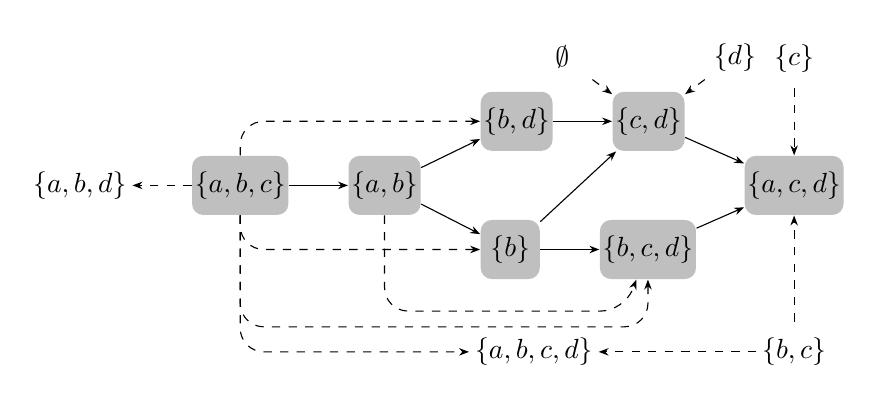
\begin{tikzpicture}[
    set/.style={inner sep=1pt, minimum size=0.75cm, align=center, fill=lightgray, rounded corners},
    otherset/.style={inner sep=2pt, minimum size=0.75cm, align=center},
    >={Stealth[scale=0.75]}
]
\node[set] (ABC) at (0,0) {$\{a,b,c\}$};
\node[set, right=0.75cm of ABC] (AB) {$\{a,b\}$};
\node[set, above right=0.05cm and 0.75cm of AB] (BD) {$\{b,d\}$};
\node[set, below right=0.05cm and 0.75cm of AB] (B) {$\{b\}$};
\node[set, right=0.75cm of BD] (CD) {$\{c,d\}$};
\node[set, right=0.75cm of B] (BCD) {$\{b,c,d\}$};
\node[set, below right=0.05cm and 0.75cm of CD] (ACD) {$\{a,c,d\}$};

\draw[->, fill=lightgray] (ABC) -- (AB);
\draw[->] (AB) -- (BD);
\draw[->] (AB) -- (B);
\draw[->] (BD) -- (CD);
\draw[->] (B) -- (BCD);
\draw[->] (B) -- (CD);
\draw[->] (CD) -- (ACD);
\draw[->] (BCD) -- (ACD);

\draw[->, dashed, rounded corners=3mm] (AB) -- ([yshift=-0.4cm]AB.south) |- ([xshift=-0.3cm, yshift=-0.4cm]BCD.south) -- ([xshift=-0.3cm]BCD);
\draw[->, dashed, rounded corners=3mm] (ABC) -- ([yshift=-0.6cm]ABC.south) |- ([yshift=-0.6cm]BCD.south) -- (BCD);
\draw[->, dashed, rounded corners=3mm] (ABC) |- (BD);
\draw[->, dashed, rounded corners=3mm] (ABC) |- (B);

\node[otherset, left=0.75cm of ABC] (ABD) {$\{a,b,d\}$};
\draw[->, dashed] (ABC) -- (ABD);

\node[otherset, below=1.35cm of ACD] (BC) {$\{b,c\}$};
\draw[->, dashed] (BC) -- (ACD);

\node[otherset, left=2cm of BC] (ABCD) {$\{a,b,c,d\}$};
\draw[->, dashed] (BC) -- (ABCD);
\draw[->, dashed, rounded corners=3mm] (ABC) |- (ABCD);

\node[otherset, above=0.85cm of ACD] (C) {$\{c\}$};
\draw[->, dashed] (C) -- (ACD);

\node[otherset, above left=0.05cm and 0.25cm of CD] (EMPTY) {$\emptyset$};
\draw[->, dashed] (EMPTY) -- (CD);
\node[otherset, above right=0.05cm and 0.25cm of CD] (D) {$\{d\}$};
\draw[->, dashed] (D) -- (CD);

\end{tikzpicture}

\end{document}